\chapter{LAMA SA-315b (truss structure)}

\section*{Introduction}
\addcontentsline{toc}{section}{Introduction}
\noindent
 The Aérospatiale Alouette II (Lama) is a French light helicopter originally manufactured by Sud Aviation that holds the distinction of being the first production helicopter to be powered by a gas turbine engine instead of the conventional heavier piston powerplant. \\
Despite being a light helicopter, the SA-315b Lama possesses a reasonable lift capacity and exceptional high altitude performances; on 21 June 1972, the type established a helicopter absolute altitude record of 12,442 m, record which remained unbroken until March 2017. \\
The Alouette II was a widely used type of helicopters with over 1,300 rotorcrafts eventually being constructed between 1956 and 1975. \\
Some versions of the Lama helicopter are still in operation in some companies (mainly used for aerial work in mountain regions) after more than 60 years from its first flight. However, in the year 2020 it is planned to be definitely retired from all the operations.

\medskip
\begin{figure}[h]
	\begin{center}
		\centering  		 		
		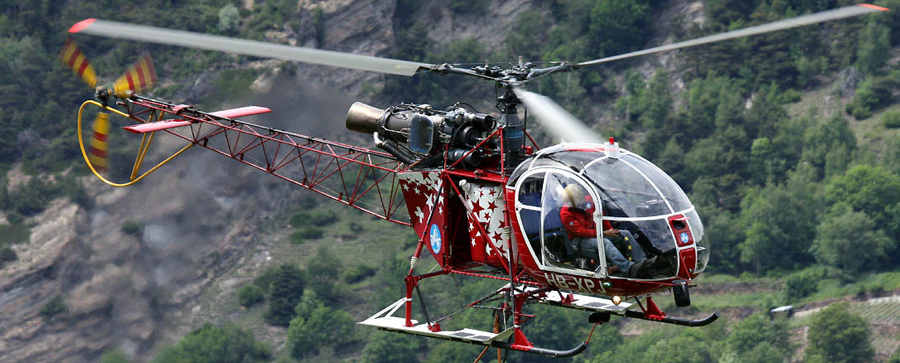
\includegraphics[width=0.95\linewidth]{PICTURES/2_Lama_truss/PNG/lama1.png}
	\end{center}
	\caption {SA-315b Lama helicopter}
\end{figure}
%\vspace{0.5cm}



\clearpage
\subsection*{General structural description }
\addcontentsline{toc}{subsection}{General structural description}
\noindent From the structural point of view the helicopter consists of three main sections: 
\begin{itemize}
	\item the cabin;
	\item the central structure;
	\item the tailboom (which is of our interest).
\end{itemize}

\noindent The central structure joins the cab with tail boom and supports dynamic components such as the turbine, the main transmission as well as commands, hydraulic controls... \\
For the airframe the manufacturer has foreseen tubular structures made of \emph{hermetically welded and interconnected steel tubes}. This solution is excellent for its simplicity and solidity and makes it easy to calculate the forces caused by traction, twist and compression. \\

\medskip
\begin{figure}[h]
	\begin{center}
		\centering  		 		
		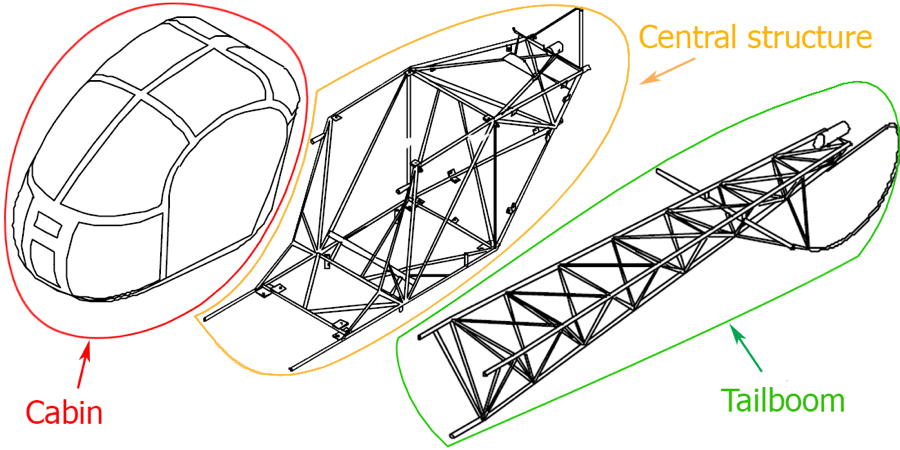
\includegraphics[width=0.8\linewidth]{PICTURES/2_Lama_truss/PNG/structure_parts.png}
	\end{center}
	\caption {Helicopter's main structural sections}
\end{figure}
\vspace{0.5cm}


\noindent INTELLIGENT SOLUTION FOR EASIER STRUCTURAL INSPECTIONS: \

\smallskip
\noindent All the airframes tubes have been designed to be filled with \textbf{Nitrogen gas under pressure} which is periodically measured in order to verify the presence of cracks or damages in some points of the structure. Furthermore, the inert gas prevent the corrosion of the structures caused by the presence of Oxygen. \\
This is undoubtedly a very intelligent and innovative solution for that time and can guarantee the safety of the flight and a long life to all the  airframe's components. \\
However, \underline{the pressure inside the tubes has been neglected in our models} cause its contribution is not so relevant from the structural and dynamical point of view.




\clearpage
\subsection*{Some useful technical specifications}
\noindent
\addcontentsline{toc}{subsection}{Some useful technical specifications}
Some data from official technical sheets and manuals will be here reported cause they have been found to be necessary to characterize some parameters of the Ansys's models and also to verify the validity of some of the obtained results. \\  


\medskip
\begin{figure}[h]
	\begin{center}
		\centering  		 		
		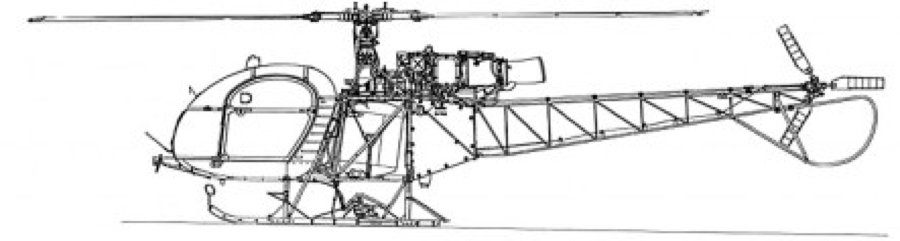
\includegraphics[width=1\linewidth]{PICTURES/2_Lama_truss/PNG/side_view.png}
	\end{center}
	\caption {SA-315b Lama technical drawing}
\end{figure}
%\vspace{0.5cm}

\smallskip
\begin{table}[h!]
	\centering
	
	\begin{tabular}{c c c c} 
		\toprule
		\multicolumn{4}{c}{Helicopter's technical parameters}\\
		\midrule
		Group & Parameter & Value & Description \\
		\midrule
		 & Length & 10.24 $[m]$  & Total helicopter's length \\
		 & Height & 3.09 $[m]$  & Max height of the helicopter \\ 
		Dimensions & $D_{main}$ & 11.02 $[m]$  & Main rotor diameter (3 blade) \\ 
		 & $A_{main}$ & 95.38 $[m^2]$ & Main rotor disk area \\  
		 & $D_{tail}$ &  1.912 $[m]$ & Tail rotor diameter (3 blade) \\ 
		 & $A_{tail}$ & 2.87 $[m^2]$ & Tail rotor disk area \\  
		 
		 
		 \midrule
		 & Max top Power & 640 $[kW]$  & Max take-off power \\
		 Engine & Max continuous Power & 440 $[kW]$  & Max continuous power \\ 
		 & Torque & 398 $[kW]$  & Max torque on transmission \\  
		
		\midrule
		
		 & $N_{engine}$ &  33500 $[RPM]$ & Engine's speed (turbine) \\
		 & $N_{output}$ &  5773 $[RPM]$ & Engine's output drive shaft \\ 
		 Speeds & $N_{rotor}$ &  353 $[RPM]$ & Main rotor normal speed \\
		 & $N_{tailrotor}$  &  2020 $[RPM]$ & Tail rotor normal speed \\ 
		 & $N_{shaft}$ &  5232 $[RPM]$ & Tailrotor's drive shaft speed \\ 
		 
			
		
		\midrule
		& $M_{empty}$ & 1021 $[kg]$  & Empty weight \\
		& $Max_{weight}$ & 2300 $[kg]$  & Max weight (with external load) \\ 
		Masses & $Engine$ & 182 $[kg]$  & Engine weight \\ 
		& $Gearbox$ & 40 $[kg]$ & Tail rotor's gearbox \\  
		& $Tail rotor$ &  25 $[kg]$ & Tail rotor weight \\  
		
		
		
		\bottomrule
	\end{tabular}
	\caption{Lama's technical parameters}
	\label{data}
	
\end{table}











\clearpage
\subsection*{Tailboom's design description (tubular)}
\addcontentsline{toc}{subsection}{Tailboom's design}
\noindent
The SA-315b Lama's tailboom structure is the airframe's part we intend to study. \\
It is composed of a trellis frame of stainless steel tubes welded together to form triangular sections connected by three main longerons that run longitudinally all the tail's length. Dimensions of the triangular sections fade out linearly along the longitudinal direction. \\
The upper horizontal cross members support the tail rotor driving shaft (fixed by bearings to the tail frame) and the tail rotor assembly which basically consist in a gearbox, a rotor hub and the blades with its hinges and actuators for yaw control. \ At the rear end there is an arched bend tube serving as a tail rotor passive protection system which prevents tail rotor from contacts with the ground or with obstacles. 

%three-quarter of the trellis there are two fixed aerodynamic surfaces joined by a transverse tube, which perform the stabilizer function during the forward flight, while at the rear

\begin{figure}[h]
	\begin{center}
		\centering  		 		
		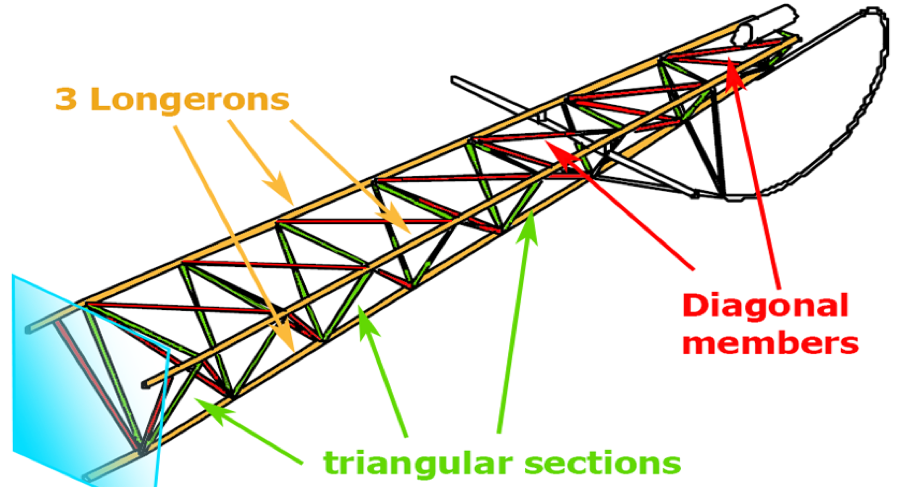
\includegraphics[width=1\linewidth]{PICTURES/2_Lama_truss/PNG/tail_written.png}
	\end{center}
	%\caption {Lama tailboom's section}
\end{figure}
%\vspace{0.5cm}

\section*{Material properties}
\noindent
Elastic isotropic materials are used in the FE model. As previously outlined, the SA315b tailboom's frame is made of staineless steel tubes welded together at the joints. The properties of the steel used for the calculations are listed in the table:

\medskip
\begin{table}[h!]
	\centering
	
	\begin{tabular}{c c c c} 
		\toprule
		\multicolumn{4}{c}{Material properties}\\
		\midrule
		Mat & Density (kg/m3) & Poisson's ratio & Young's modulus (GPa) \\
		\midrule
		Steel & 7850  &  0.29 & 205 \\ 
		\bottomrule
	\end{tabular}	
\end{table}


\clearpage
\subsection*{Tubes real constants and properties}
\addcontentsline{toc}{subsection}{Tubes real constants and material properties}

\noindent
Airframe's tubes have all been modelled using BEAM elements with hollow circle cross sections (CTUBE) which have different real constants depending on type of the tube. \\ Property of the sections used in the model as well as the formula used to perform the calculations are listed in the following tables. 

\bigskip
\begin{figure}[h]
	\begin{center}
		\centering  		 		
		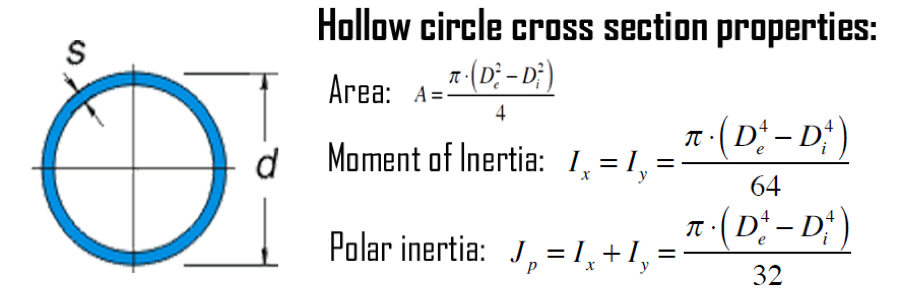
\includegraphics[width=0.9\linewidth]{PICTURES/2_Lama_truss/PNG/tube1.png}
	\end{center}
	\caption {Tube's cross section}
\end{figure}
%\vspace{0.5cm}


\medskip
\begin{table}[h!]
	\centering
	
	\begin{tabular}{c c c c} 
		\toprule
		\multicolumn{4}{c}{Tubes cross section's properties}\\
		\midrule
		Family & Parameter & Value & Description \\
		\midrule
		& $\phi_{ext}$ &  \textbf{28} $[mm]$ & External diameter \\
		& $s$ &  \textbf{2} $[mm]$ & Tube's thickness \\ 
		Longerons & $A_{section}$  &  163 $[mm^2]$ & Area of the cross section \\ 
		& $I_{x} = I_{y}$ &  $13885.8$ $[mm^4]$ & Moment of inertia \\ 
		& $I_{p}$ &  $6942.9$ $[mm^4]$ & Polar moment of inertia \\
		

		\midrule
		& $\phi_{ext}$ &  \textbf{12} $[mm]$ & External diameter \\
		& $s$ &  \textbf{1.5} $[mm]$ & Tube's thickness \\ 
		Cross elements & $A_{section}$  &  49.5 $[mm^2]$ & Area of the cross section \\ 
		& $I_{x} = I_{y}$ &  $695.8$ $[mm^4]$ & Moment of inertia \\ 
		& $I_{p}$ &  $347.9$ $[mm^4]$ & Polar moment of inertia \\
		
		
		\midrule
		& $\phi_{ext}$ &  \textbf{12} $[mm]$ & External diameter \\
		& $s$ &  \textbf{1.5} $[mm]$ & Tube's thickness \\ 
		Diagonal elements & $A_{section}$  &  49.5 $[mm^2]$ & Area of the cross section \\ 
		& $I_{x} = I_{y}$ &  $695.8$ $[mm^4]$ & Moment of inertia \\ 
		& $I_{p}$ &  $347.9$ $[mm^4]$ & Polar moment of inertia \\
		
			
		\bottomrule
	\end{tabular}
	\caption{Tailboom's technical parameters}
	
\end{table}

\noindent
In this case it is possible to use the default generalized cross-sections included in the Ansys "SECTYPE" command of the beam elements.




\clearpage
\section*{Approach to the problem}
\section{Basic structure model (airframe only)}
\subsection*{Analysis model}
\addcontentsline{toc}{subsection}{Analysis model}
\noindent
A fully parametric model of the truss tail boom has been developed in Ansys APDL language on the base of the technical drawings found on the aircraft's official manuals and reported in the appendix. Some missing dimensions have been recovered from a scaled CAD model of the same helicopter type developed by model aircraft's builders. \\
The model has been developed using a \emph{bottom-up approach} creating the necessary key-points and lines and then meshing the elements. Additional local reference frames have been used to simplify the geometry definition. \\
The following picture outline the main features of the naked structure's model. \\

 \medskip
 \begin{figure}[h]
 	\begin{center}
 		\centering  		 		
 		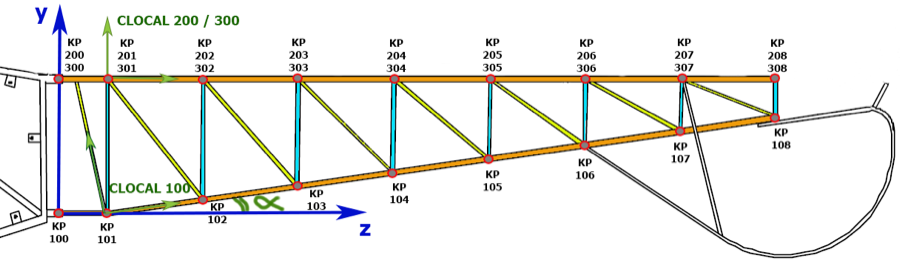
\includegraphics[width=1\linewidth]{PICTURES/2_Lama_truss/PNG/tail_complete_mod.png}
 	\end{center}
 	\caption {Tailboom's analysis model (truss)}
 \end{figure}
 %\vspace{0.5cm}
 
 \bigskip
 \begin{table}[h!]
 	\centering
 	
 	\begin{tabular}{c c c} 
 		\toprule
 		\multicolumn{3}{c}{Tailboom's main parameters}\\
 		\midrule
 		Parameter & Value & Description \\
 		\midrule
 		Lt & 4.8 $[m]$  & Total tail length \\
 		L1 & 0.7 $[m]$  & Equilateral triangular section side lenght (at the root) \\ 
 		L5 & 0.075 $[m]$  & Half width of the tail at the tip (along x axis) \\ 
 		w1 & 0.48 $[m]$ & z-coordinate of KP 101 (Lt/10) \\  
 		alpha &  10 $[deg]$ & Angle of inclination of the lower longeron \\

 		\bottomrule
 	\end{tabular}
 	\caption{Problem's data}
 	
 \end{table}

\clearpage
\subsection*{Model assumptions}
\addcontentsline{toc}{subsection}{Model assumptions}

\noindent
\begin{quoting}
	\begin{itemize}
		
		\item Element type: \textbf{BEAM 189}, a quadratic 3-node element in 3D with 6 dofs for each node and based on Timoshenko beam theory which includes shear-deformation effects;
		
		\item uniform cross-sections of the elements along the tail's length;
		
		\item \underline{linear elastic isotropic} material properties;
		
		\item self-weight of the elements considered;
		
		\item geometrical non-linearities included in the static analysis (NLGEOM,ON) \\
		
	\end{itemize}
\end{quoting}

 \smallskip
\subsection*{Tailboom model (airframe only)}

\begin{figure}[h]
	\begin{center}
		\centering  		 		
		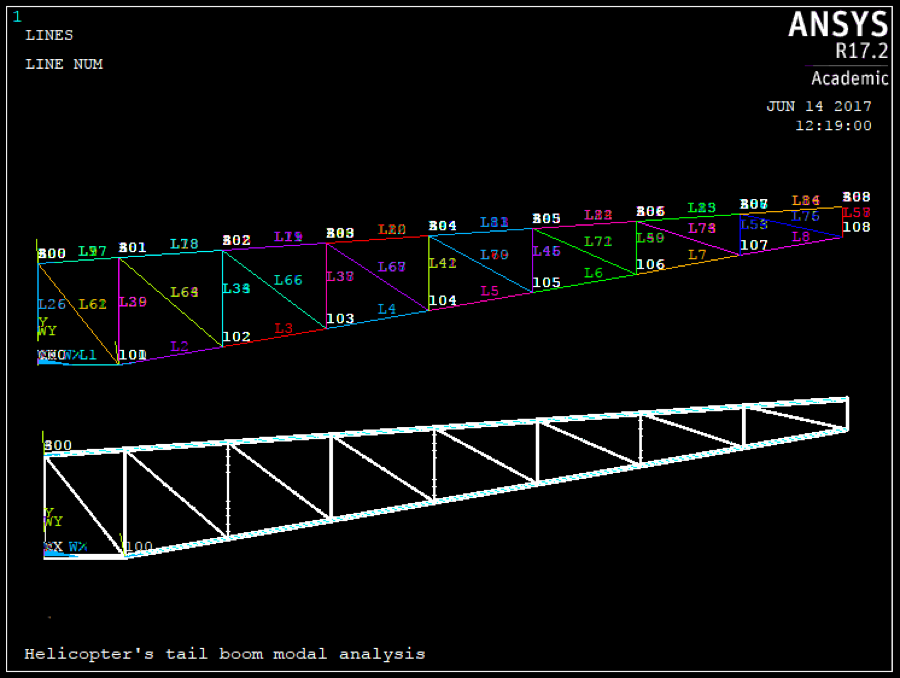
\includegraphics[width=1\linewidth]{PICTURES/2_Lama_truss/PNG/model_1_mod.png}
	\end{center}
	\caption {Analysis model (truss) side view}
\end{figure}
\vspace{0.5cm}



\noindent
Isometric views of the model in which it is possible to see the keypoints generated and the lines representing the beam's axes as well as the resulting elements. 
 \smallskip
\begin{figure}[h!]
	\begin{center}
		\centering  		 		
		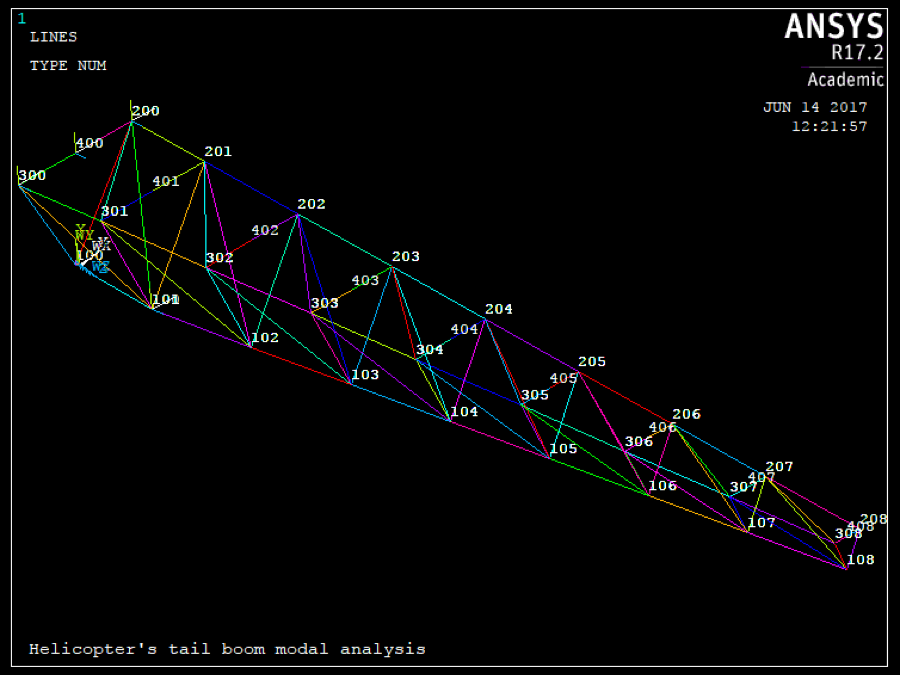
\includegraphics[width=0.79\linewidth]{PICTURES/2_Lama_truss/PNG/model_2.png}
	\end{center}
	\caption {Structure of the model - (3D view)}
\end{figure}
%\vspace{0.5cm}

\smallskip
\begin{figure}[h!]
	\begin{center}
		\centering  		 		
		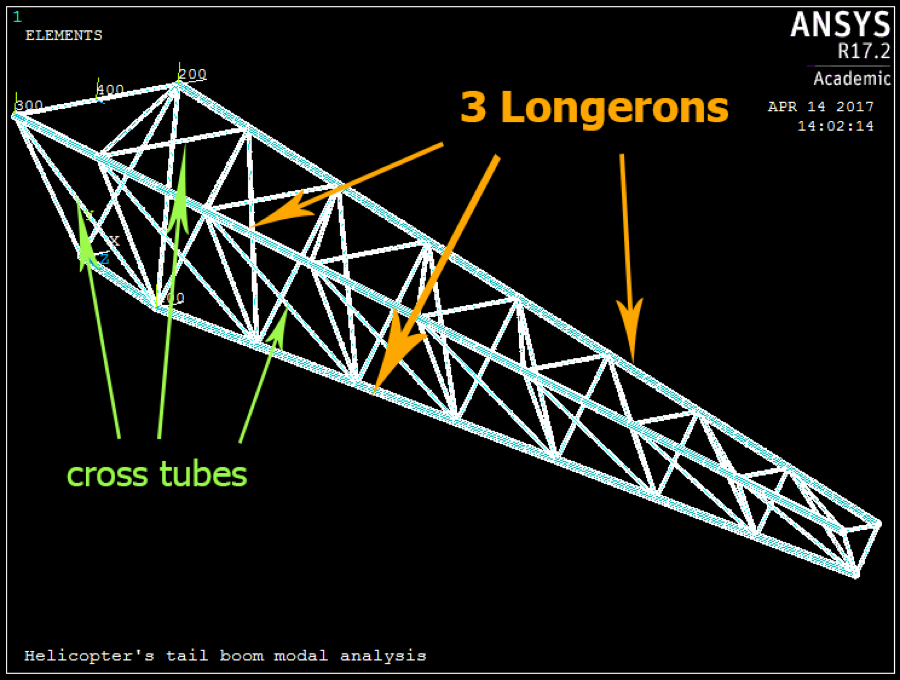
\includegraphics[width=0.79\linewidth]{PICTURES/2_Lama_truss/PNG/beam_ISO2.png}
	\end{center}
\end{figure}
%\vspace{0.5cm}
 


\clearpage
\subsection*{Applied loads for static analysis}
\addcontentsline{toc}{subsection}{Applied loads for static analysis}
\noindent
To verify the model by means of a preliminary static analysis we just considered the effect of the \textbf{self-weight} of the structure and the contribution of the \textbf{thrust (Ty)} which is provided by the tail rotor to balance the maximum applied torque by the motor. 

\smallskip
\begin{figure}[h!]
	\begin{center}
		\centering  		 		
		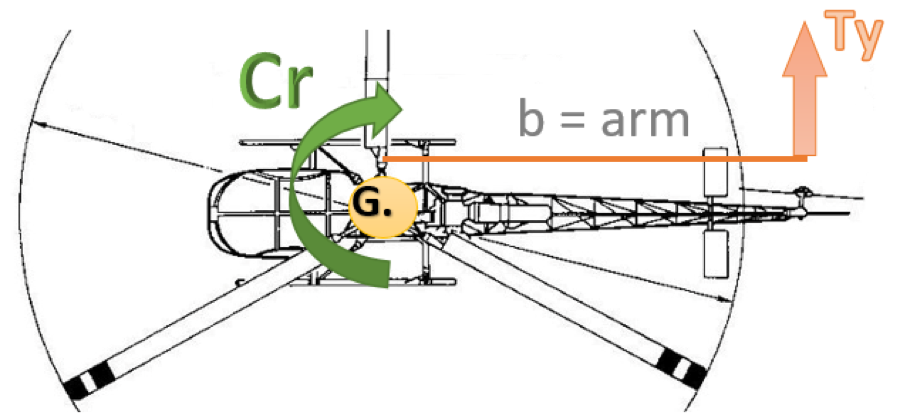
\includegraphics[width=0.79\linewidth]{PICTURES/2_Lama_truss/PNG/anticoppia.png}
	\end{center}
\end{figure}
%\vspace{0.5cm}

\noindent
ASSUMPTIONS: 
\begin{itemize}
	\item Ty is orthogonal to the plane of rotation of the tail rotor;
	\item It is computed from helicopter's technical data considering its maximum value corresponding to the maximum torque applied to the main rotor by the transmission;
	\item Cr is the reaction torque equal to the Cm (maximum motor torque) because of the third newton law. 
	\item Aerodynamic forces, inertial and centrifugal accelerations due to manoeuvres during flight are not taken into account.
\end{itemize}

\noindent
The equations used to compute the value of the force are:
\begin{equation*}
Torque (N*m) \, \, = \, \, \frac{Power \, \, absorbed(W)}{head \, \, speed(rad/s)}  
\end{equation*}

\begin{equation*}
C_m  = \frac{W}{\omega} \, = \, \frac{398000 (W)}{36.966 (rad/s)} \, = \, 10767 (Nm)
\end{equation*}
where W is the main rotor maximum power absorbed, while $\omega$ is the main rotor head speed. \
The tail rotor thrust required can be computed from the following eq. :

\begin{equation*}
C_r = T_y * b \, \, \, \, \, => \, \, \, \, \,  Ty = \frac{C_r}{b} \, = \, \frac{10767(Nm)}{4.8 (m)}  \, = \, \textbf{2243} \, (N)
\end{equation*}



\clearpage
\subsection*{Applied boundary conditions}
\addcontentsline{toc}{subsection}{Applied boundary conditions}
\noindent
According to the literature, helicopter's vibrations, caused by the main rotor assembly, are usually analyzed by assuming the response of the fuselage to react in a similar manner to that of a 'free-free' beam. \\
However, our interest is limited at the study of a part of the entire structure, the tailboom; this requires a different investigation procedure. \\ 
For the project's purposes, the tail boom can be satisfactorily modelled as a beam structure which is rigidly clamped at the large cockpit mass so it can be seen as a fixed-free beam. \\





\smallskip
\begin{figure}[h!]
	\begin{center}
		\centering  		 		
		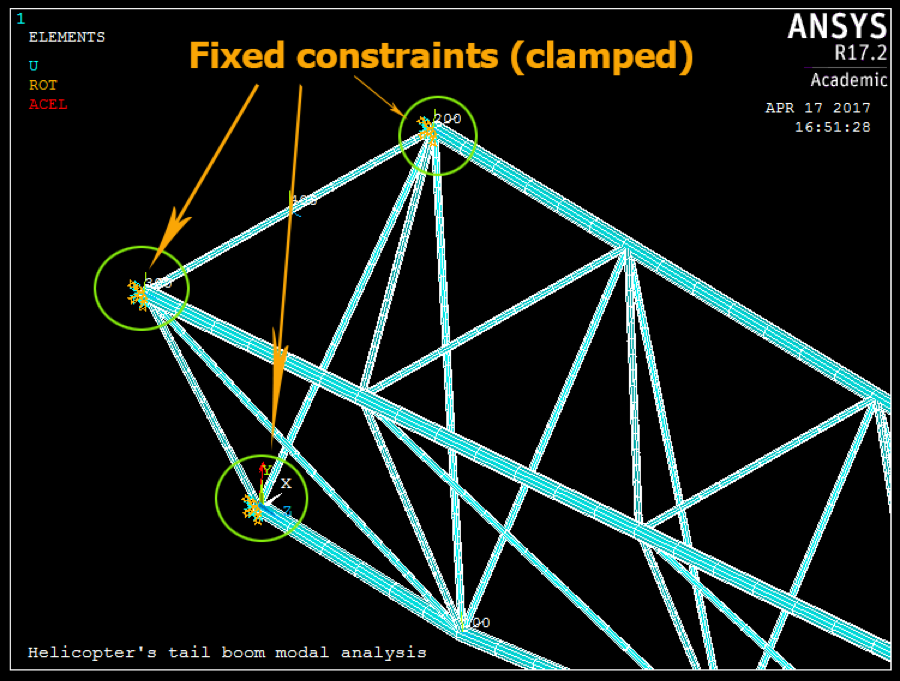
\includegraphics[width=0.8\linewidth]{PICTURES/2_Lama_truss/PNG/BC.png}
	\end{center}
	%\caption{Model's boundary conditions}
\end{figure}	
%\vspace{0.5cm}

\smallskip
\begin{figure}[h!]
	\begin{center}
		\centering  		 		
		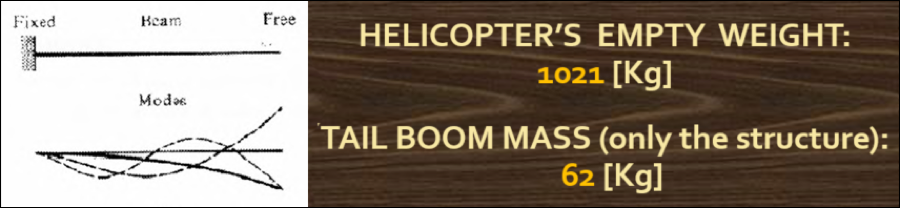
\includegraphics[width=1\linewidth]{PICTURES/2_Lama_truss/PNG/BC1.png}
	\end{center}
\end{figure}	
%\vspace{0.5cm}

\noindent
NODES AT THE ROOT of the tail -> ALL dofs (displacements and rotations) locked; \\
TAIL ROTOR THRUST FORCE -> applied at the tail tip node and acts orthogonally.


\clearpage
\subsection*{Preliminary static solution (model checking)}
\addcontentsline{toc}{subsection}{Preliminary static solution}
\noindent
At the very beginning, a preliminary static analysis has been done in order to check the \textbf{effectiveness} of the FEM model developed. 
In this step, geometrical non-linearities (stress-stiffening effects) has been included (command "NLGEOM,ON") and the optimized default options to find the non linear solutions has been also activated ("SOLCONTROL,ON"). After this step, the model is ready to be solved.

\subsubsection*{PLDISP and PLNSOL (node's displacement)}
%\smallskip
\begin{figure}[h!]
	\begin{center}
		\centering  		 		
		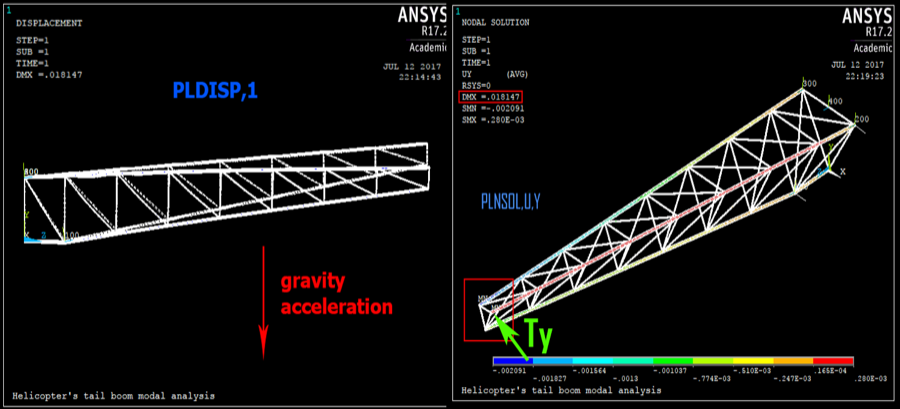
\includegraphics[width=0.95\linewidth]{PICTURES/2_Lama_truss/PNG/displ.png}
	\end{center}
	%\caption{Model's boundary conditions}
\end{figure}	
%\vspace{0.5cm}

\subsubsection*{Reactions at constrained nodes PRRSOL}
%\smallskip
\begin{figure}[h!]
	\begin{center}
		\centering  		 		
		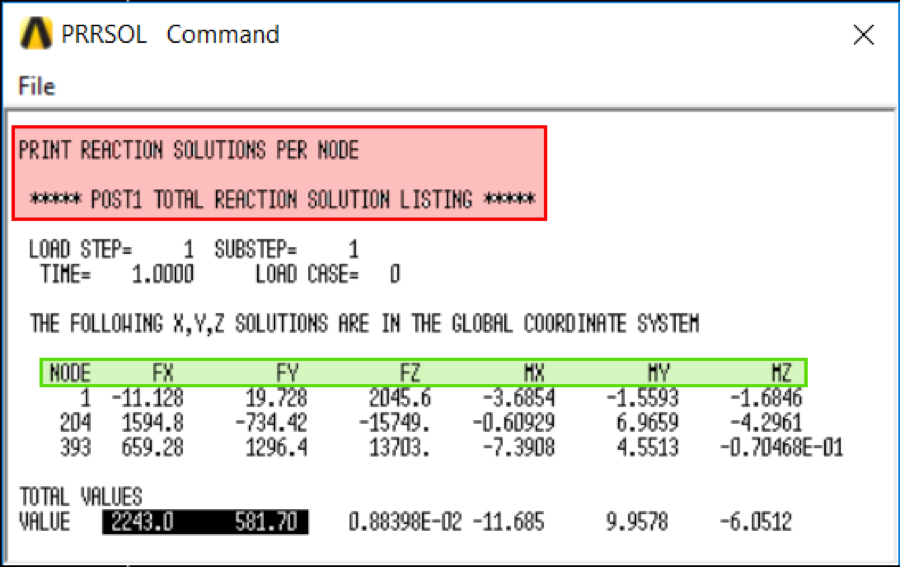
\includegraphics[width=0.65\linewidth]{PICTURES/2_Lama_truss/PNG/PRRSOL.png}
	\end{center}
	%\caption{Model's boundary conditions}
\end{figure}	
%\vspace{0.5cm}
\noindent
Results match with the self-weight (vertical) and the tail thrust (horizontal) forces applied. 
\clearpage



\clearpage
\section*{Modal Analysis (airframe only)}
\addcontentsline{toc}{subsection}{Modal Analysis (airframe only)}
\noindent
Modal analysis is a technique used to determine the structure's vibration characteristics (vibration modes) in terms of \textbf{natural frequencies}, \textbf{modal shapes} and eventually \textbf{mode partecipation factors}. \\
This is one of the project's scopes aimed to dynamically characterize the structure. \\

\noindent
\underline{ASSUMPTIONS}:
\begin{itemize}
	\item free vibration (forces, pressures...are ignored in modal analysis);
	\item no damping (it effect on $\omega_{n}$ is negligible);
	\item synchronous harmonic motions.  
\end{itemize}

\smallskip
\noindent
The approach consists to solve an EIGENVALUE PROBLEM in order to compute the resonant frequencies (eigenvalues) and modal shapes (eigenvectors) of the characteristic polynomial by means of \emph{suitable algorithms}. 

\medskip
\begin{figure}[h!]
	\begin{center}
		\centering  		 		
		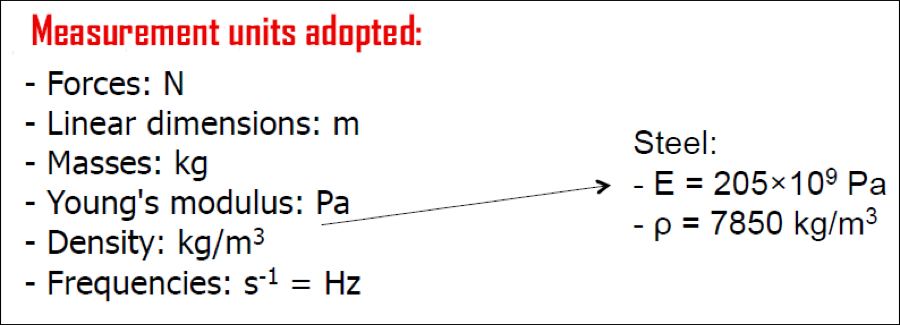
\includegraphics[width=0.8\linewidth]{PICTURES/2_Lama_truss/PNG/MU.png}
	\end{center}
	\caption{Note on measurement units adopted}
\end{figure}	
%\vspace{0.5cm}

%\smallskip
\begin{figure}[h!]
	\begin{center}
		\centering  		 		
		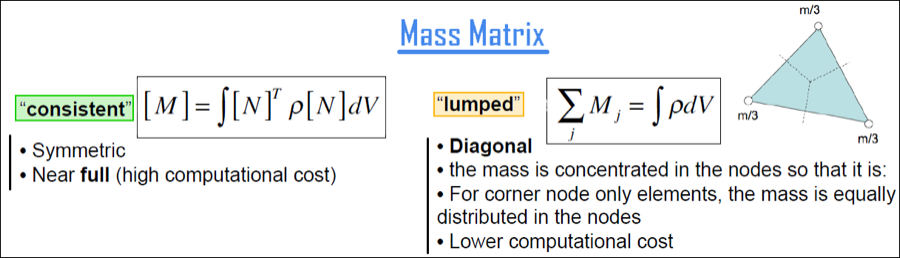
\includegraphics[width=1\linewidth]{PICTURES/2_Lama_truss/PNG/CL1.png}
	\end{center}
	\caption{Note on consistent and lumped mass matrix formulation}
\end{figure}	
%\vspace{0.5cm}


\clearpage
\subsubsection*{Note on the real tubes masses}
\noindent
The shapes and frequencies are directly dependent on the mass and stiffness properties of the elements of the structure. Hence, the masses of the tubes are an important parameter in the computations regarding the modal analysis. To be accurate in modelling, the real \emph{weight per meter mass} of the tailboom's tubes have been found from the manufacturer and have been loaded as a material parameter using the ADDMASS option of the beam elements SECCONTROL command that allows to specify the value of the real weight of the tubes per unit length. 

\subsubsection*{Model checking}
\noindent
The total mass of the taiboom frame has been computed from the Ansys model in order to check the consistency of the model developed with respect to the real aircraft's data. \\
The value of the mass of the taiboom without the additional subsystems results in 62.5 kg which matches the expected mass estimated from the real technical data.
\begin{figure}[h]
	\begin{center}
		\centering  		 		
		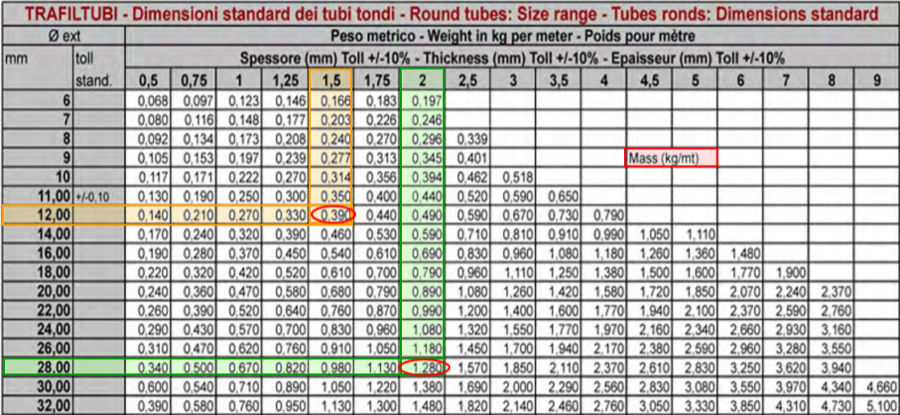
\includegraphics[width=1\linewidth]{PICTURES/2_Lama_truss/PNG/addmass2.png}
	\end{center}
	\caption {Tubes weight per unit length}
\end{figure}
%\vspace{0.5cm}




\begin{figure}[h]
	\begin{center}
		\centering  		 		
		
\includegraphics[width=0.8\linewidth]{PICTURES/2_Lama_truss/PNG/tot_mass.png}
	\end{center}
	\caption {Tubes weight per unit length}
\end{figure}
%\vspace{0.5cm}


\clearpage
\subsection*{Analysis type and options}
\noindent
\begin{figure}[h]
	\begin{center}
		\centering  		 		
		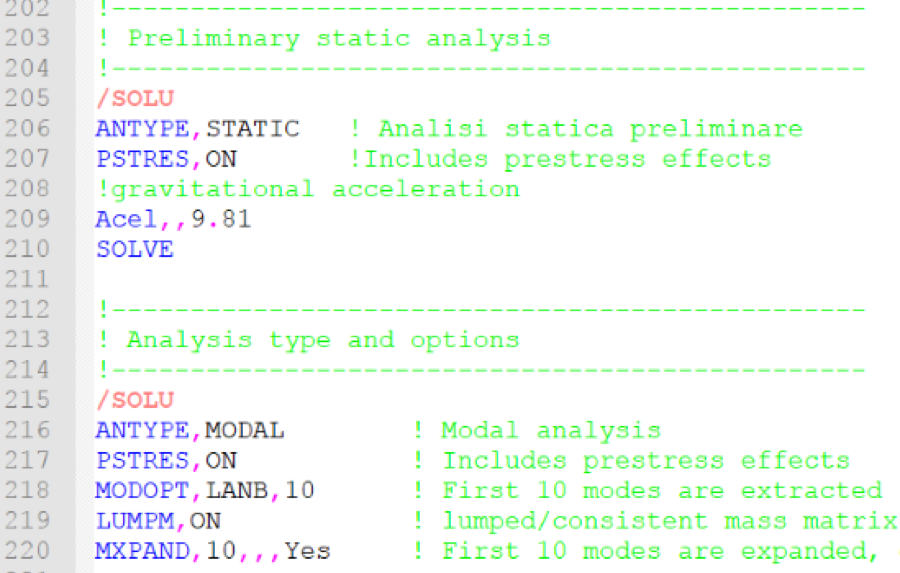
\includegraphics[width=0.9\linewidth]{PICTURES/2_Lama_truss/PNG/antype2.png}
	\end{center}
\end{figure}


\subsection*{Convergence analysis}
\noindent
\begin{figure}[h]
	\begin{center}
		\centering  		 		
		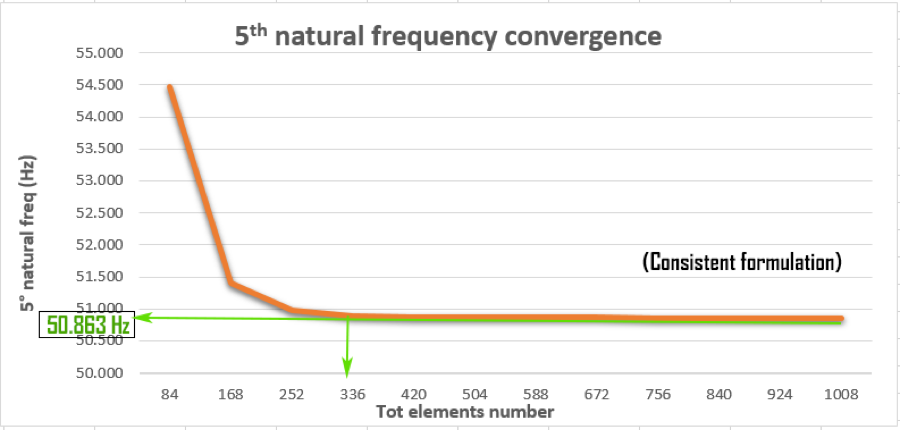
\includegraphics[width=0.8\linewidth]{PICTURES/2_Lama_truss/PNG/cov.png}
	\end{center}
	\caption {Convergence analysis on the 5th natural frequency}
\end{figure}



\subsection*{Resonant frequencies}
\noindent
The first 10 resonant frequencies obtained at the end of the convergence analysis are now displayed in the following results table:
\begin{figure}[h]
	\begin{center}
		\centering  		 		
		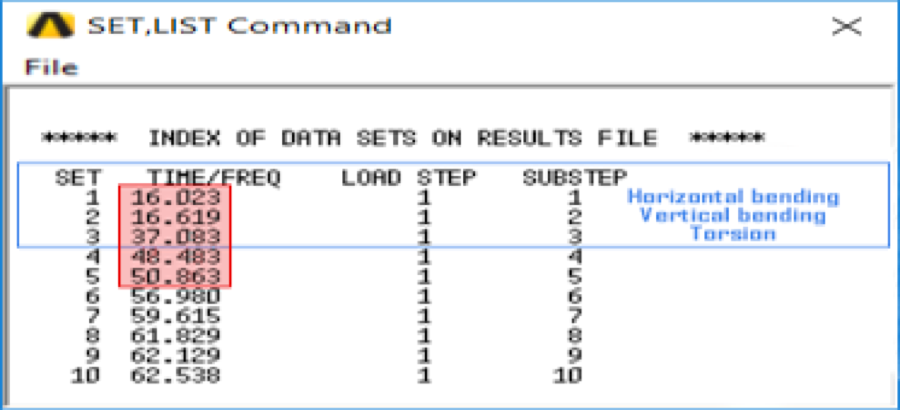
\includegraphics[width=0.70\linewidth]{PICTURES/2_Lama_truss/PNG/set-list.png}
	\end{center}
	%\caption {List the first 10 computed natural frequencies}
\end{figure}

\subsection*{First 4 modal shapes}
\noindent
Eigenvectors are typically normalized in Ansys with respect to the mass matrix and; this normalization is very useful from the computational point of view. However, the drawback is that in this way they represent correctly the shape of the mode but not the real amplitude of the displacement which in turn depends on the initial conditions. 

\begin{figure}[h]
	\begin{center}
		\centering  		 		
		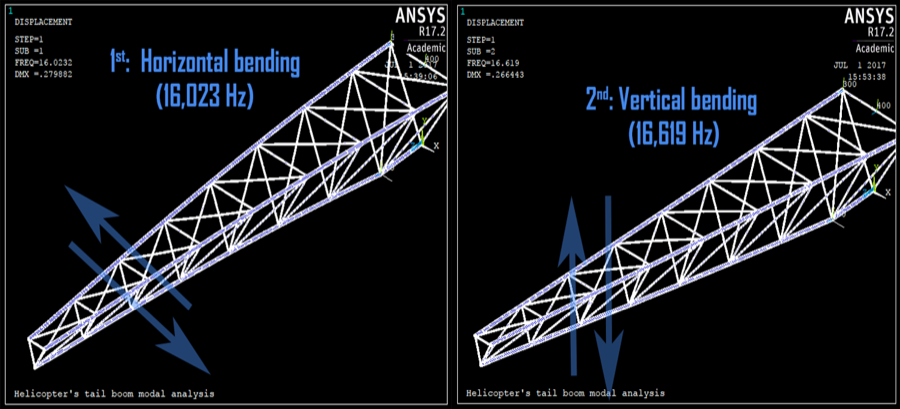
\includegraphics[width=0.95\linewidth]{PICTURES/2_Lama_truss/PNG/1-2.png}
	\end{center}
	\caption {Graphical representation of the first and second modal shapes}
\end{figure}

\noindent
The first three mode shapes are related to the \emph{horizontal,vertical and torsional} movement of the tailboom. The fourth shows a node at the rear three quarter of the tail while higher order modes are related to tubes movements at higher frequencies. 

\begin{figure}[h]
	\begin{center}
		\centering  		 		
		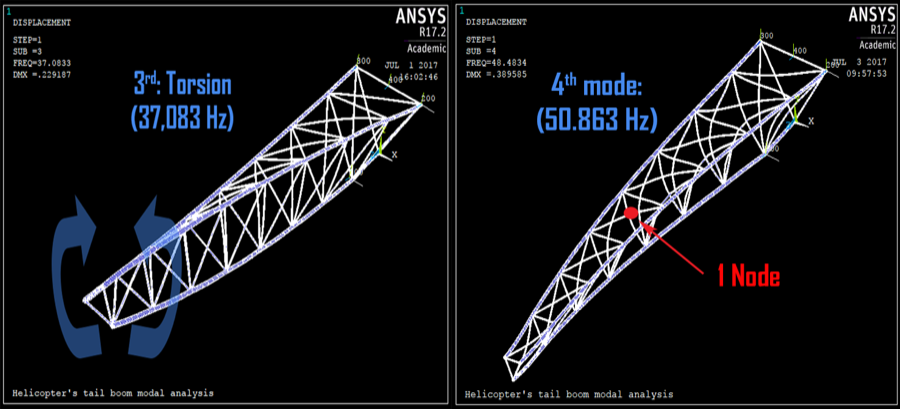
\includegraphics[width=0.95\linewidth]{PICTURES/2_Lama_truss/PNG/3-4.png}
	\end{center}
	\caption {Graphical representation of the third and fourth modal shapes}
\end{figure}


%\clearpage
\subsection*{Results comparison with literature}
\noindent
In order to have a reference about the results obtained from Ansys, our computed tailboom's natural frequencies have been compared with those found in the literature. Serendipitously, dimensions and materials of the helicopter's model analyzed in the paper are comparable to our model and also the results found at the end of the convergence analysis reasonably match with those reported in the literature (maximum 5 \% difference) at least for the first three vibration modes. \\
\begin{figure}[h]
	\begin{center}
		\centering  		 		
		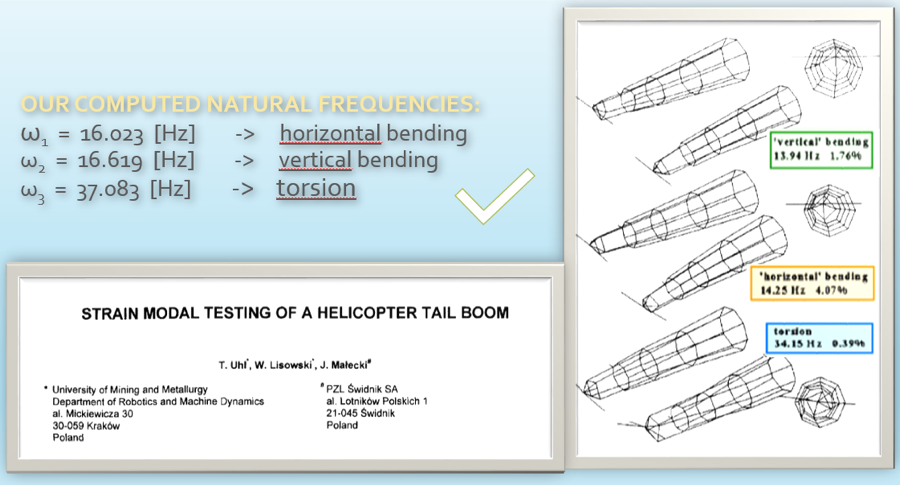
\includegraphics[width=1\linewidth]{PICTURES/2_Lama_truss/PNG/comparison.png}
	\end{center}
	%\caption {Results comparison with literature data found}
\end{figure}

\clearpage
\section{Fully parametric model (airframe + subsystems)}
\noindent
At this point only the naked tailboom's airframe has been studied. It is necessary to model also the subsystems fixed on it in order to perform an accurate characterization of the dynamic behaviour of the whole real system. \\
The additional components present on an helicopter tail are basically:
\begin{itemize}
	\item the \underline{tail rotor's driving shaft} and the bearings that support it;
	\item the tail rotor assembly composed of the \underline{rotor hub}, \underline{blades} and the 90 degrees \underline{gearbox};
	\item aerodynamic surfaces such as the \underline{horizontal stabilizers};
	\item an \underline{arched bend tube} serving as a tail rotor passive protection system.
\end{itemize}



\smallskip
\begin{figure}[h!]
	\begin{center}
		\centering  		 		
		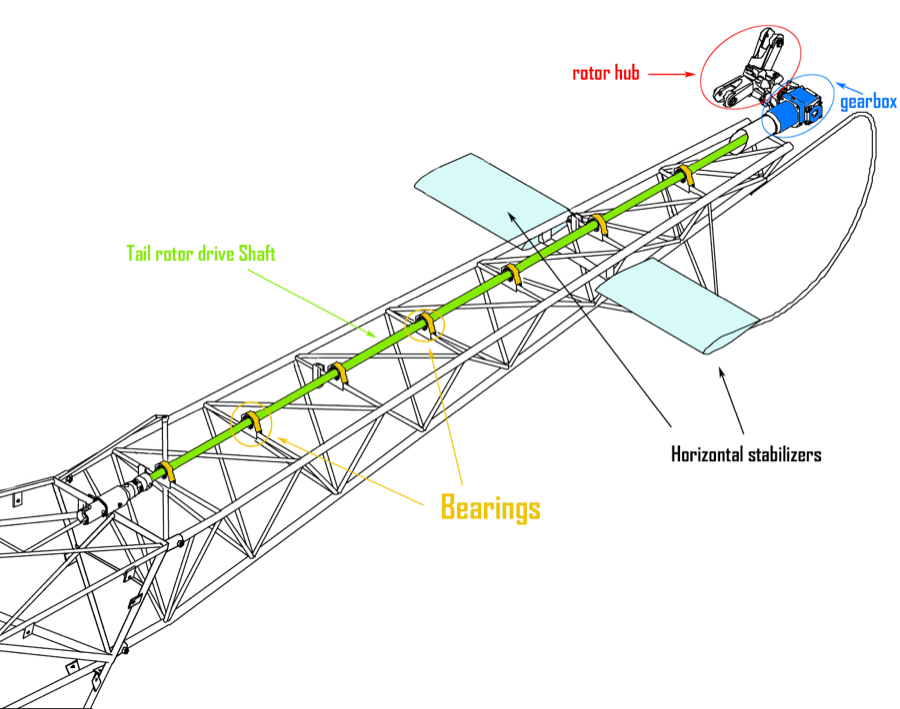
\includegraphics[width=1\linewidth]{PICTURES/2_Lama_truss/PNG/model2/tail_complete_2.png}
	\end{center}
	%\caption{Additional subsystems}
\end{figure}	
%\vspace{0.5cm}

\noindent
For our purposes, the horizontal stabilizers have been considered only as concentrated masses neglecting the aerodynamic forces they produce since we are considering a stationary (hover) fly condition whereas the rotor protection tube has been, instead, neglected. 

\clearpage
\subsection*{Tail rotor's drive shaft}
\noindent
The Tail Rotor drive system receives the energy from the engine and consists in two parts (a forward drive shaft attached directly to the engine and a longer rear drive shaft) which are both connected to each other, to the engine and to the Tail Gear Box by 3 \emph{flexible couplings} to allow lateral and vertical motions of the tailboom. \\
The very long tail rotor drive shaft is supported by 7 ball bearing support assemblies mounted on rubber bushes that damp out the vibrations.

\smallskip
\begin{figure}[h!]
	\begin{center}
		\centering  		 		
		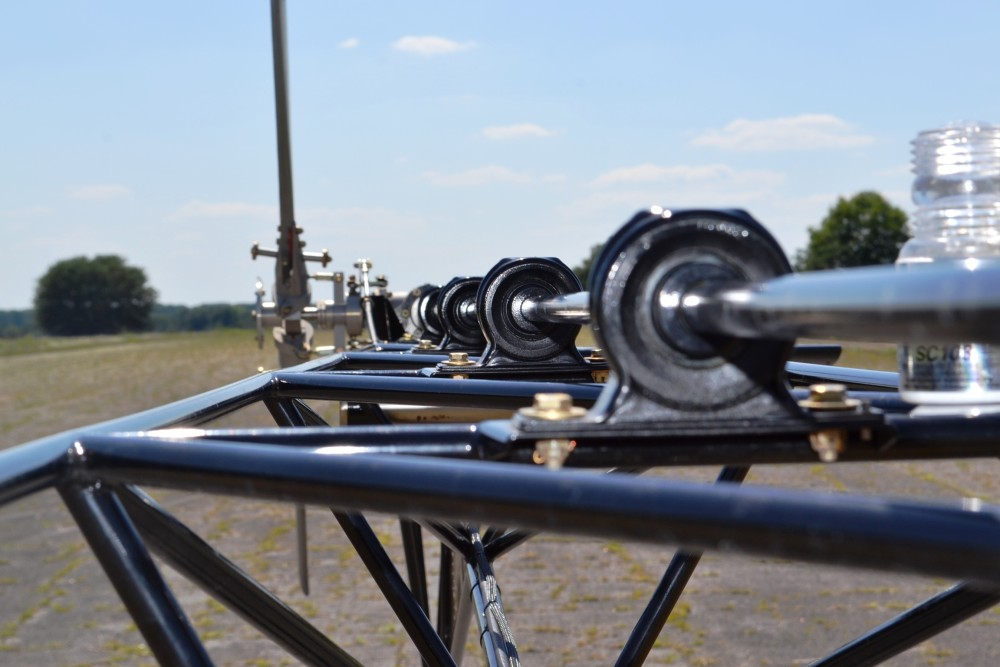
\includegraphics[width=0.85\linewidth]{PICTURES/2_Lama_truss/PNG/model2/driveshaft}
	\end{center}
	\caption{Tail rotor drive shaft bearing supported}
\end{figure}	
%\vspace{0.5cm}

\medskip
\begin{table}[h!]
	\centering
	
	\begin{tabular}{c c c c c} 
		\toprule
		\multicolumn{5}{c}{Shaft's properties}\\
		\midrule
		Material & type & Density (kg/m3) & Poisson's ratio & Young's modulus (GPa) \\
		\midrule
		Ergal & serie 7075 & 2810  &  0.33 & 72 \\ 
		\midrule
		\\
		\midrule
		Part & length (m) &   & N° of segments & dimension (m) \\
		\midrule
		Entire shaft length & 4.8 &   & 8  &  0.6  \\ 
		\bottomrule
	\end{tabular}	
\end{table}

\noindent 
The shaft's mass is about 7 kg; however, considering bearings, flexible joints and additional components to fix the shaft along the tail's length, the total mass rises up to \textbf{12 kg} which are considered equally distributed on the 7 point masses located along the tail.
\clearpage
\subsection*{Gearbox}
\noindent
The Tail Gear Box is basically an angle reduction gear for mounted in and protected by a steel casing filled with oil for lubrication purpose. Its weight is around \textbf{30 kg}. \
The transmission ratio is about 2.59 and it contributes to reduce the rotational speed from 5232 RPM of the shaft to the 2020 RPM of the tail rotor hub. \\
The gearbox is connected to the tail boom structure by 3 bolts and which \emph{represent the main interface from which forces, moments and displacements are transferred}. \\

\smallskip
\begin{figure}[h!]
	\begin{center}
		\centering  		 		
		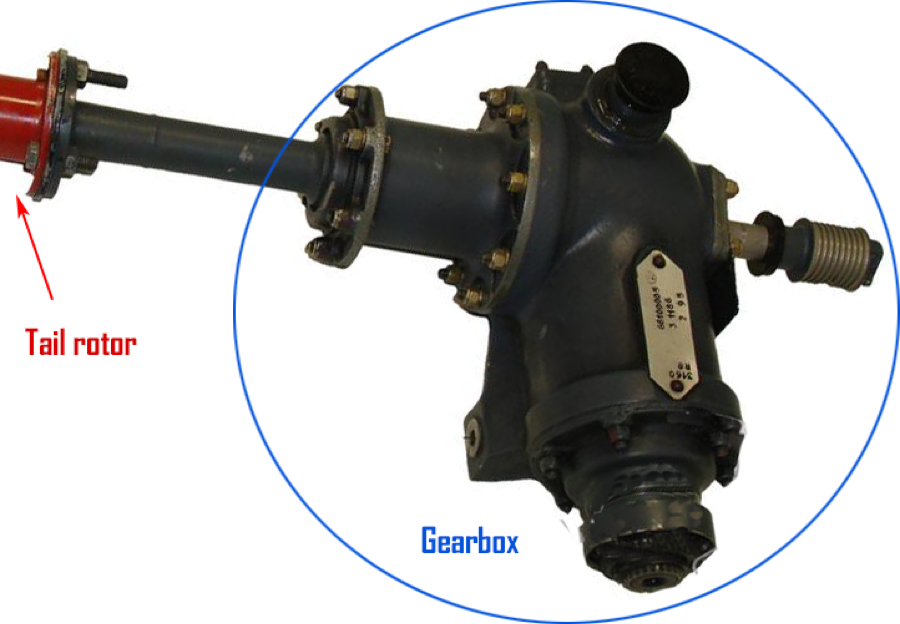
\includegraphics[width=0.8\linewidth]{PICTURES/2_Lama_truss/PNG/model2/gearbox}
	\end{center}
	\caption{90 degrees gearbox}
\end{figure}	
%\vspace{0.5cm}

\medskip
\begin{figure}[h!]
	\begin{center}
		\centering  		 		
		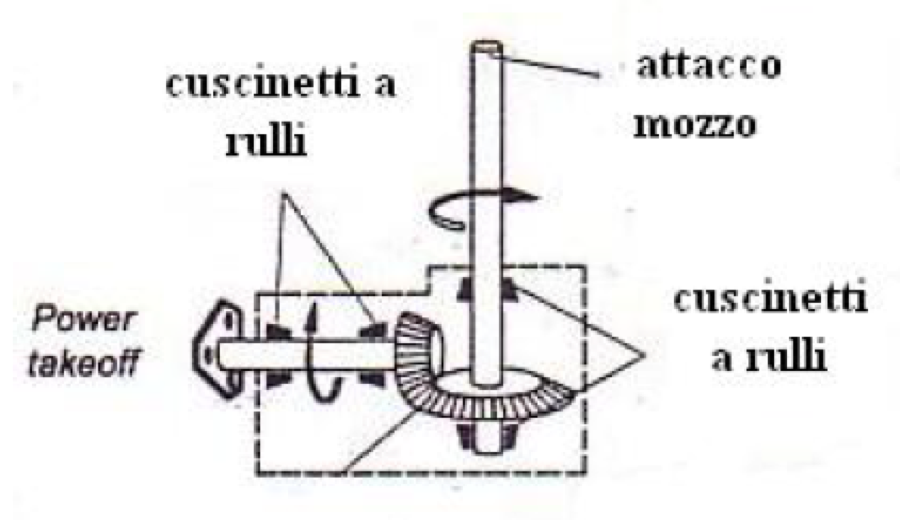
\includegraphics[width=0.65\linewidth]{PICTURES/2_Lama_truss/PNG/gearbox_tail_scheme}
	\end{center}
	%\caption{90 degrees gearbox}
\end{figure}	
%\vspace{0.5cm}


\bigskip
\subsection*{Rotor assembly (hub + blades)}
\noindent
The rotor assembly is composed of a \underline{rotor hub}, \underline{3 blades} and a \underline{shaft} which is connected to the gearbox from one side and it sustain the hub and the blades on the other end. 

\medskip
\begin{table}[h!]
	\centering
	
	\begin{tabular}{c c c c c} 
		\toprule
		\multicolumn{5}{c}{Rotor's assembly properties}\\
		\midrule
		Item & components & Mass (kg) & Polar inertia (kg $m^2$) & Length (m) \\
		\midrule
		Hub & 1 & 30  &  1.776  & / \\ 
		\midrule
		Blades & 3 & 5 each  & / & 0.596 \\
		\midrule
		Shaft & 1 & 1  &  /  & 0.5 \\
		
		\bottomrule
	\end{tabular}	
\end{table}


\smallskip
\begin{figure}[h!]
	\begin{center}
		\centering  		 		
		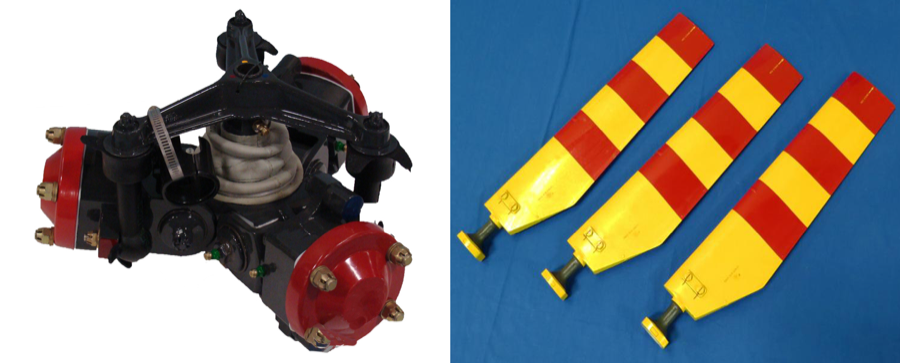
\includegraphics[width=0.9\linewidth]{PICTURES/2_Lama_truss/PNG/model2/hubeblades}
	\end{center}
	\caption{Tail rotor hub and blades}
\end{figure}	
%\vspace{0.5cm}

\subsubsection*{Rotor's concentrated inertia}
\noindent
Blades are modelled as thin rectangular beams ( $I_{blade} = \frac{1}{12} m L^2 $ w.r.t its center of mass).
To consider the inertia respect to the root of the blade, we can use Huygens-Steiner theorem:
\begin{equation*}
I_{root} = I_{CoM} + m_{blade}  \left( \frac{L}{2} \right) ^2  \, = \, 0.59 \, \, (kg \, m^2)
\end{equation*}

\begin{equation*}
I_{rotor} = n_{blades} * I_{root} \, = \,  \textbf{1.776} \, \, (kg \, m^2)
\end{equation*}

\noindent
In literature, as first approximation, tail rotor is considered as a rigid disk fixed on a beam's shaft supported by two elastic bearings. \\
For our purposes, the tail rotor assembly has been modelled considering the \underline{rotor hub} as a \textbf{concentrated mass and inertia} located at the shaft's tip node.




\clearpage
\section*{Modal Analysis (complete model)}
\addcontentsline{toc}{subsection}{Modal Analysis (complete model)}

\begin{figure}[h!]
	\begin{center}
		\centering  		 		
		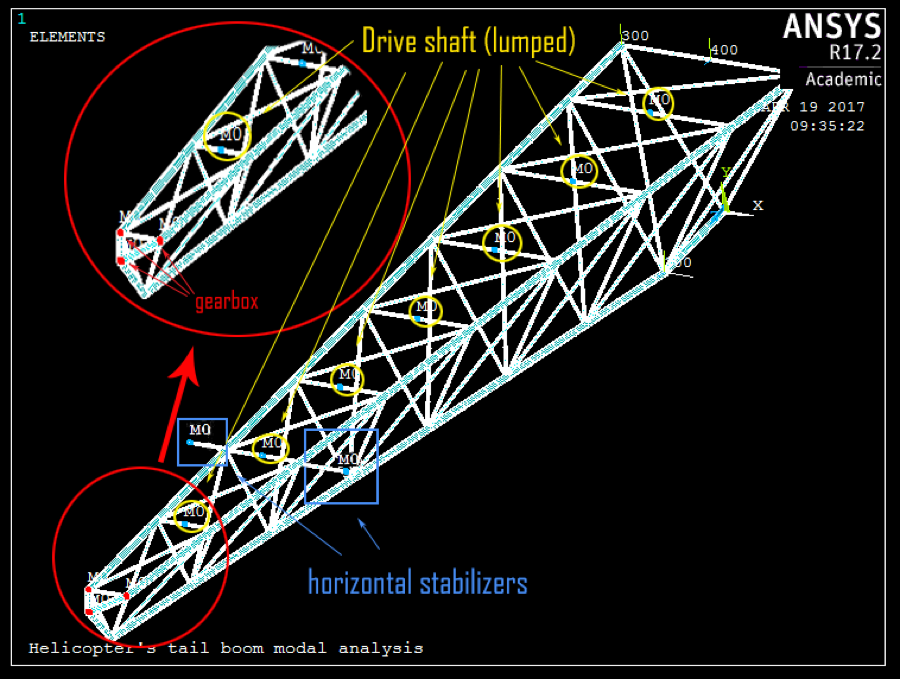
\includegraphics[width=0.9\linewidth]{PICTURES/2_Lama_truss/PNG/model2/lumped_approach1.png}
	\end{center}
	\caption{Additional subsystems}
\end{figure}	
%\vspace{0.5cm}



\subsection*{Applied boundary conditions}
\addcontentsline{toc}{subsection}{Applied boundary conditions}
\noindent
The helicopter structure can be modelled to first approximation as a large point mass (the main rotor assembly and cockpit) connected by the relatively slender tail boom to a small point mass (the tail rotor assembly). Because of this significant difference in mass, the tail boom can be satisfactorily modelled as a beam structure which is rigidly clamped at the large cockpit mass and has an end mass equal to that of the tail rotor assembly. \\

\smallskip
\begin{figure}[h!]
	\begin{center}
		\centering  		 		
		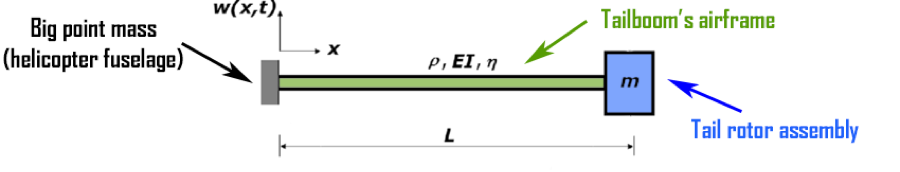
\includegraphics[width=0.95\linewidth]{PICTURES/2_Lama_truss/PNG/BC0.png}
	\end{center}
	%\caption{First approximation model of the tailboom}
\end{figure}	
%\vspace{0.5cm}


\clearpage
\subsection*{Full model's natural frequencies}
\noindent
Again, the first 10 resonant frequencies of the full model, obtained at the end of the convergence analysis, are displayed in the following results table:
\begin{figure}[h!]
	\begin{center}
		\centering  		 		
		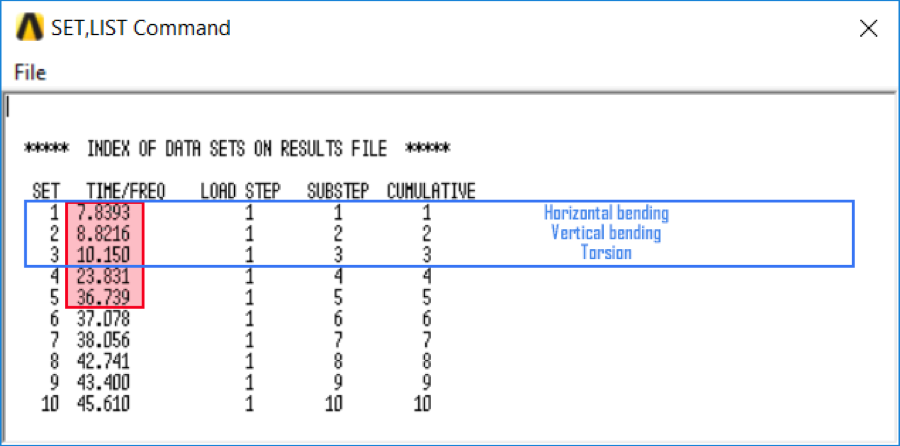
\includegraphics[width=0.70\linewidth]{PICTURES/2_Lama_truss/PNG/model2/set-list2.png}
	\end{center}
	\caption {List the first 10 computed natural frequencies computed}
\end{figure}
\noindent
As the case of the simple model, the first three regards the case of horizontal, vertical bending and torsion but they results to be lowered down. This fact match with our expectation since the \underline{subsystems} \underline{add weight and inertia to the whole structure shifting down its dynamical behaviour} toward lower frequencies.
Tu sum up, the following picture represents the results obtained for the simple and complete truss airframe models. 
\begin{figure}[h!]
	\begin{center}
		\centering  		 		
		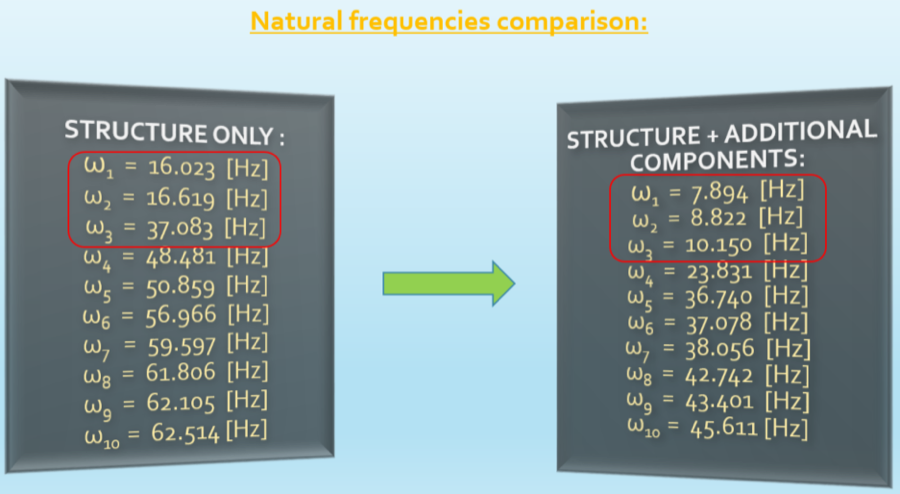
\includegraphics[width=0.70\linewidth]{PICTURES/2_Lama_truss/PNG/model2/comparison.png}
	\end{center}
	%\caption {List the first 10 computed natural frequencies computed}
\end{figure}

\smallskip
\noindent
IMPORTANT NOTE: \\
At this stage, those resonant frequencies are computed without considering the tail-rotor rotation. To consider the dynamic effects linked to the rotation of the system we must perform a \emph{tailrotor-fuselage coupled analysis}, as introduced in the chapter 4. \\ 






















\clearpage
\bigskip